\documentclass[12pt,aspectratio=169]{beamer}

% Input
\usepackage[utf8]{inputenc}
\usepackage[T1]{fontenc}
\usepackage[letterspace=100]{microtype}
\usepackage{upquote}

% Beamer
\usetheme{metropolis}
\usepackage[sfdefault]{FiraSans}
\usepackage{xcolor}
\definecolor{blue}{HTML}{002957}
\definecolor{red}{HTML}{F1563F}
\setbeamercolor{palette primary}{fg=white,bg=blue}
\setbeamercolor{title separator}{fg=red,bg=blue}
\setbeamercolor{frametitle}{fg=white,bg=blue}
\setbeamercolor{progress bar}{fg=red,bg=blue}
\setbeamercolor{alerted text}{fg=red,bg=blue}
\makeatletter
\setlength{\metropolis@titleseparator@linewidth}{2pt}
\setlength{\metropolis@progressonsectionpage@linewidth}{2pt}
\setlength{\metropolis@progressinheadfoot@linewidth}{2pt}
\makeatother

% Graphics
\usepackage{graphicx}
\usepackage{epstopdf}
\DeclareGraphicsExtensions{.png,.pdf,.eps}
\tikzset{
  invisible/.style={opacity=0},
  visible on/.style={alt={#1{}{invisible}}},
  alt/.code args={<#1>#2#3}{%
    \alt<#1>{\pgfkeysalso{#2}}{\pgfkeysalso{#3}} % \pgfkeysalso doesn't change the path
  },
}
\usetikzlibrary{arrows, shapes}

% Various
\usepackage{hyperref}
\usepackage{minted}
\usepackage{fontawesome}
\usepackage{multicol}
\usepackage[normalem]{ulem}

% Title
\title{Camunda Chapter: Finland}
\date{12.6.2024}
\author{Asko Soukka}
\institute{\vspace{1cm}
\includegraphics[height=1.5cm]{images/jyu-vaaka-kaksikielinen.eps}}

\newcommand{\setmytemplate}{}

\newcommand\Wider[2][1cm]{%
\makebox[\linewidth][c]{%
  \begin{minipage}{\dimexpr\textwidth+#1\relax}
  \raggedright#2
  \end{minipage}%
  }%
}

\begin{document}

%---------------------------------------------------------------------------------------

\setbeamertemplate{footline}[plain]
\setbeamertemplate{background canvas}[default]
\maketitle

%---------------------------------------------------------------------------------------

\setbeamercolor{background canvas}{bg=white}
\setbeamertemplate{footline}{}

\begin{frame}{}
  \vspace{1cm}
  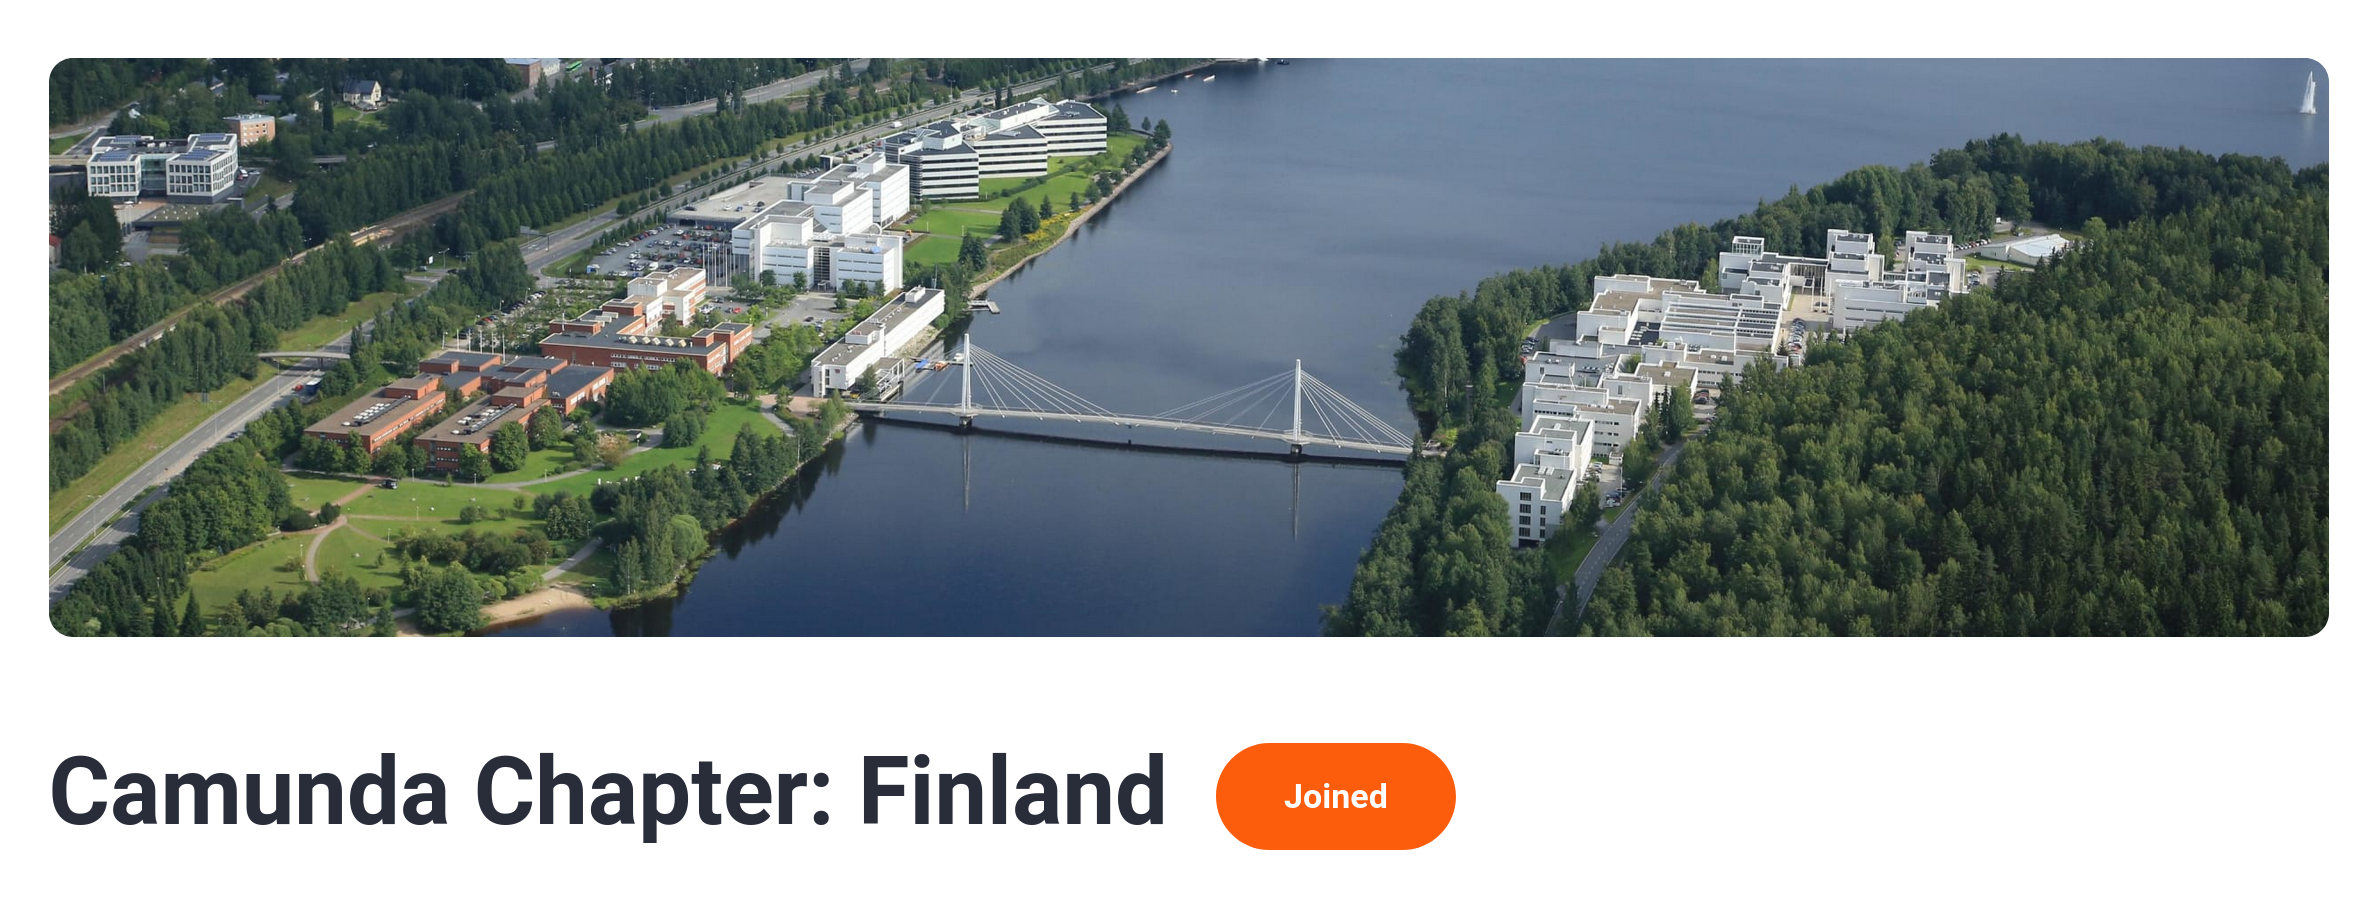
\includegraphics[width=0.875\paperwidth]{images/camunda-chapter-finland.png}
  \vspace{-1cm}
  \begin{itemize}[]
  \item[] 2024-06-12 @ 1400–-1600 EEST:
  \item BPMN ja pienet avuliaat elinkaariprosessit
  \item BPMN.io elementtimallit (\textit{Element Templates})
  \end{itemize}
\end{frame}

\setbeamertemplate{background canvas}[default]
\begin{frame}[standout]
\begin{minipage}{0.4\textwidth}
\begin{itemize}[]
  \item[] Camunda
  \item[] Chapter:
  \item[] Finland
\end{itemize}
\end{minipage}
\begin{minipage}{0.5\textwidth}
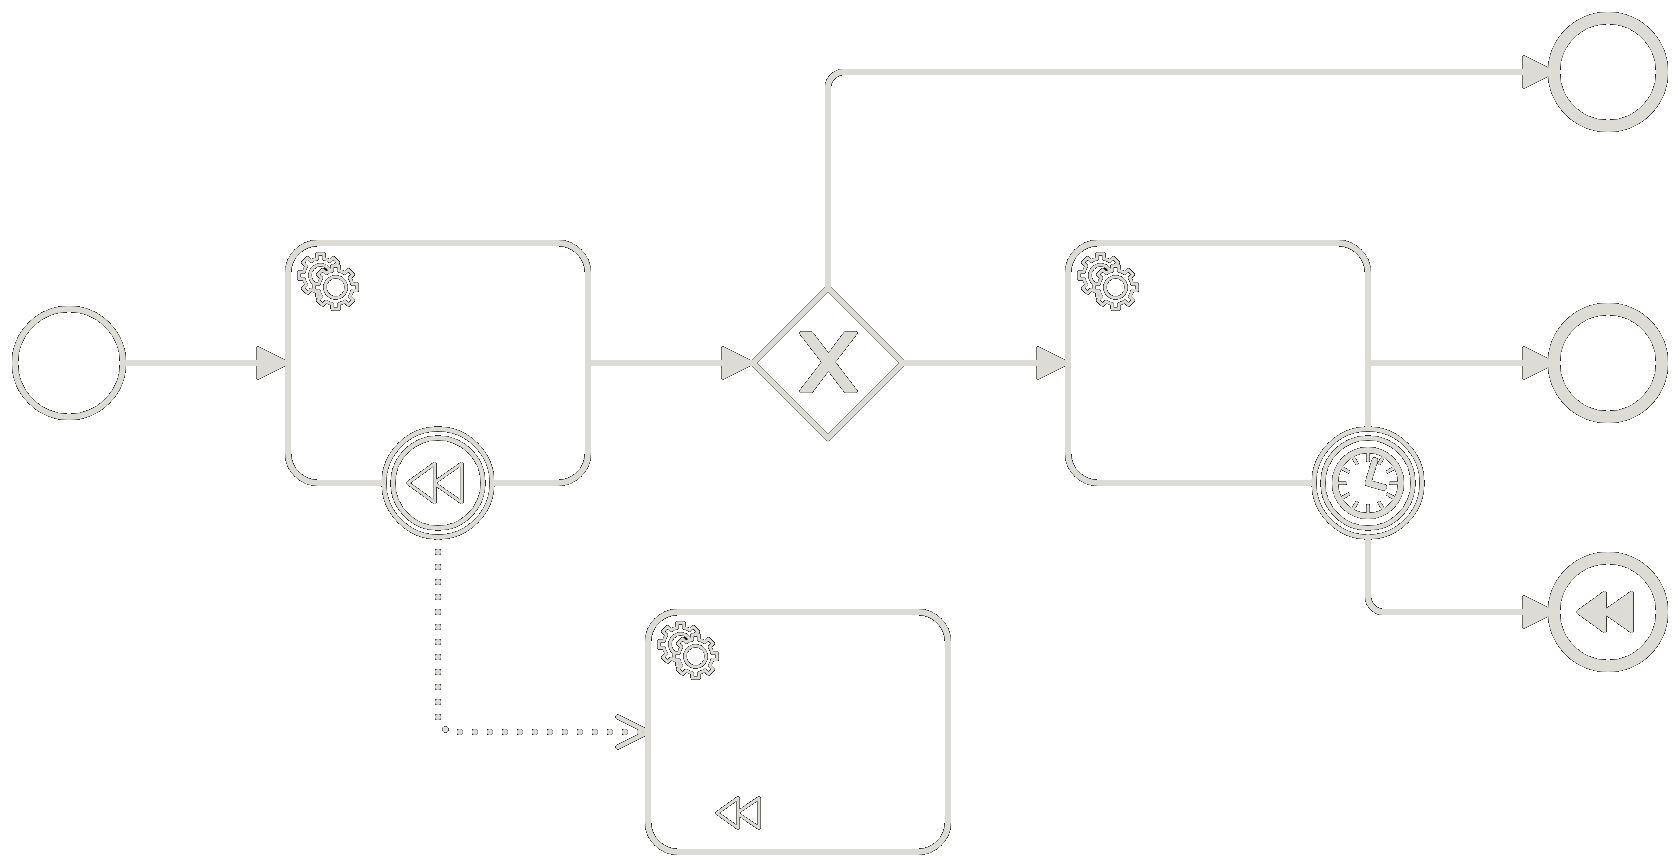
\includegraphics[width=0.8\paperwidth]{images/bpmn-example.png}
\end{minipage}
\end{frame}

\setbeamertemplate{background canvas}[default]
\begin{frame}[standout]
\begin{minipage}{0.4\textwidth}
\begin{itemize}[]
  \item[] University of Jyväskylä
  \item[]
  \item[] Digital Services
\end{itemize}
\end{minipage}
\begin{minipage}{0.5\textwidth}
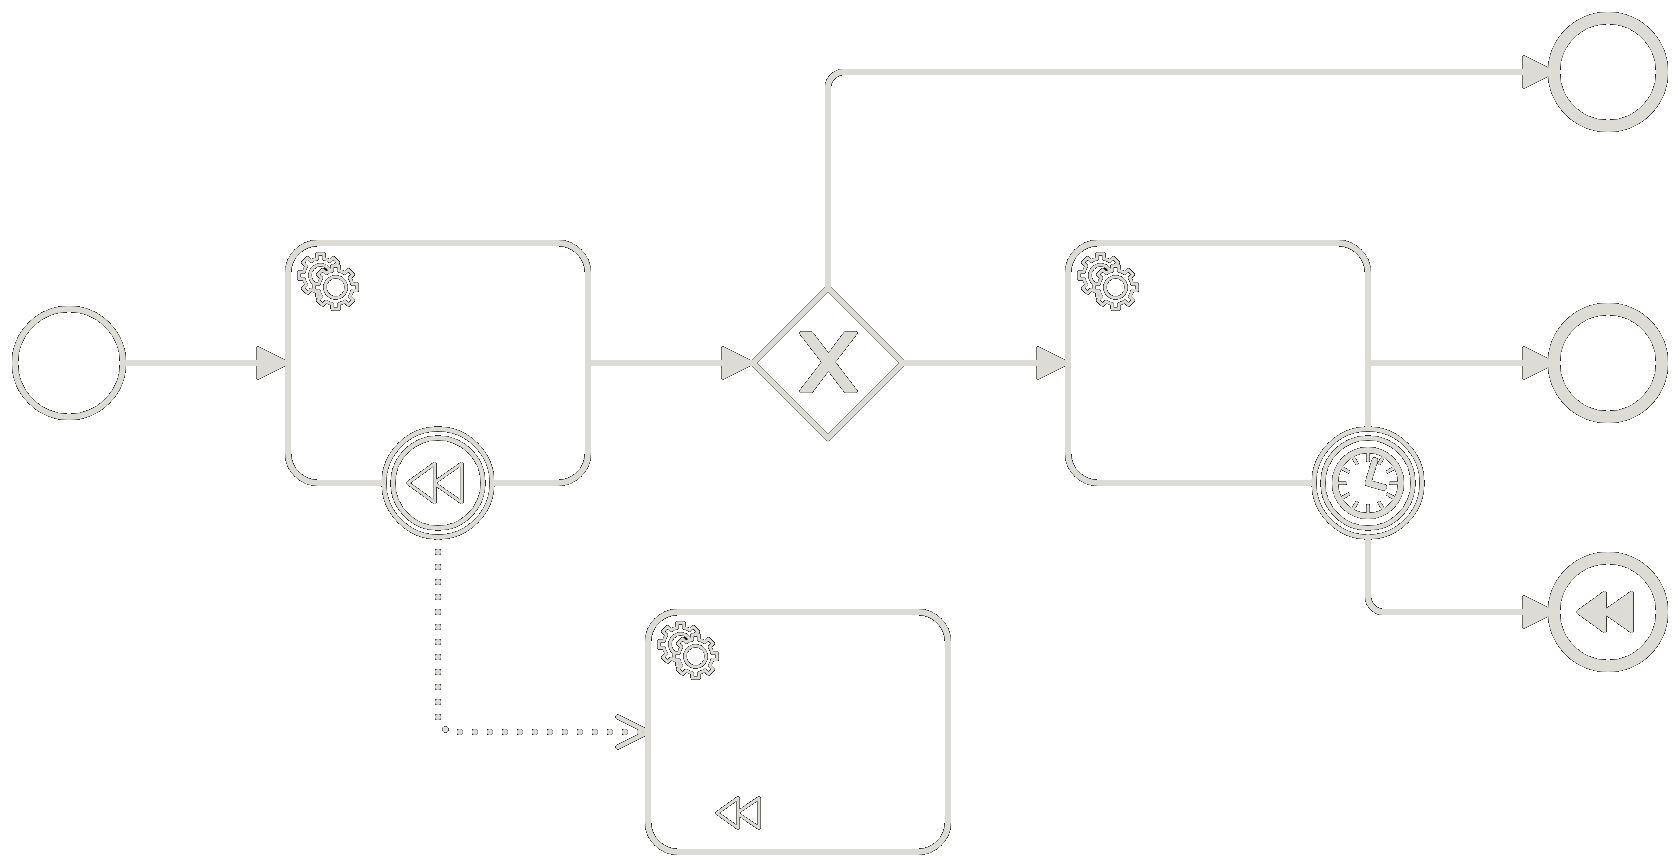
\includegraphics[width=0.8\paperwidth]{images/bpmn-example.png}
\end{minipage}
\end{frame}

\setbeamertemplate{footline}[plain]
\setbeamertemplate{background canvas}[default]

%% \section{Agenda}

\begin{frame}{2024-06-12 @ 1400–1600 CEST}
\begin{minipage}{0.5\textwidth}
\begin{itemize}[]
    \item[] 1400–
    \item[] \textbf{BPMN ja pienet avuliaat elinkaariprosessit}
    \item[] Asko Soukka, JY
    \item[] Pasi Anttonen, JY
\end{itemize}
\end{minipage}
\begin{minipage}{0.45\textwidth}
\begin{itemize}[]
    \item[] 1500–
    \item[] \textbf{BPMN.io elementtimallit}
    \item[] Asko Soukka, JY
    \item[]
    \item[]
\end{itemize}
\end{minipage}
    \vspace{0.5cm}
\begin{itemize}[]
    \item[] 1530–
    \item[] \textbf{META ja keskustelua}
\end{itemize}
\end{frame}

\end{document}
